%
% quantenfeldtheorie.tex -- Quantenfeldtheorie: Quantisierung, Schrödinger-Gleichung, der harmonische Oszillator, Photonen als Oszillatoren
%
% (c) 2020 Prof Dr Andreas Müller, Hochschule Rapperswil
%
% !TEX root = ../../buch.tex
% !TEX encoding = UTF-8
%
\section{Quantenfeldtheorie\label{fourier:section:quantenfeldtheorie}}
\kopfrechts{Quantenfeldtheorie}
Zwei grundlegende Begriffe der Quantenfeldtheorie sind Quant und Quantisierung. 
Ein Quant ist ein kleinst mögliches Teilchen und Quantisierung bedeutet nichts anderes als zählbar. 
In der Quantenfeldtheorie ist genau dieser Schritt von zentraler Bedeutung, denn nun ist alles zählbar. 
Dabei werden klassische Felder wie das elektromagnetische Feld in quantenmechanische Operatoren überführt, wodurch die zuvor kontinuierlichen Felder plötzlich aus einer endlichen Menge von Quanten bestehen.
Wie kam es eigentlich dazu, dass man physikalische Grössen plötzlich als „quantisiert“ betrachtete?
Ein kurzer Blick in die Geschichte hilft, diesen Schritt besser zu verstehen.

\subsection{Die Idee der Quantisierung\label{fourier:subsection:DieIdeeDerQuantisierung}}
	Mit 16 Jahren fragte Max Planck seinen Physiklehrer, ob sich ein Studium in der Physik lohne. 
	Dieser soll geantwortet haben, dass im Fach im Grunde schon alles entdeckt sei und nur noch ein paar Lücken zu füllen blieben.
	Das war 1874.
	Zum Glück liess sich Planck davon nicht abhalten.
	1897 wurde er Professor für Physik und beschäftigte sich mit einem dieser ungelösten Probleme, der Schwarzkörperstrahlung. 
	
	
	In der Abbildung~\ref{fourier:fig:schwarzkoerper} ist das Experiment dargestellt. Ein hohler Metallwürfel mit einem Loch wird erwärmt. 
	Die ganze elektromagnetische Strahlung, die von aussen in das Loch eindringt, wird im Inneren absorbiert und ist visualisiert durch den blauer Pfeil. 
	Die austretende Strahlung wird nur vom Würfel Inneren abgegeben, siehe die roten Pfeile. 
	Der schwarze Strahler ist in Wirklichkeit das Loch und nicht das Material selbst, obschon man dazu ein geeignetes Material benötigt! Nun misst man welche Intensität von welcher Wellenlänge aus dem Loch ausdringt, diese hängt auch von der Temperatur des Metallwürfel ab. 
	
	Gut zu wissen ist, dass jedes Objekt über dem absoluten Nullpunkt elektromagnetische Wellen abstrahlt. 
	Sehen tut man dies bei Raumtemperatur nicht, da die Strahlungintensität im sichtbaren Wellenbereich, zwischen 400nm und 780nm, extrem gering ist. 
	Erst bei höheren Temperaturen wird die strahlung für uns sichtbar. 
	
	\input{papers/fourier/fig/fig-schwarzkoerper.tex}
	
	In der Abbildung~\ref{fourier:fig:strahlungsspektren} wurde der Metallblock auf 1000K erwärmt und anschliessend gemessen, wie hoch die Intensität bei jeder Wellenlänge ist. 
	Die Messwerte liegen auf der schwarzen Kurve.
	Bei dieser Temeratur glüht das Eisen rötlich, hiermit handelt es sich um vom Bock abgegebene elektromagnetische Strahlung!
	
	
	Nach dem Rayleigh-Jeans-Gesetz 
	
	\begin{equation}
		B(\lambda, T) = \frac{2 \pi c k_\mathrm{B} T}{\lambda^4}
	\end{equation}
	
	steigt die abgegebene Strahlungintensität eines Körpers mit kleiner werdender Wellenlänge immer weiter an. 
	Bei hohen Wellenlängen passt das Gesetz gut, aber im ultravioletten Bereich versagt die Theorie komplett. Ultraviolette Strahlung umfasst den Wellenbereich von 10 nm bis 400 nm. 
	Die Formel sagt gigantische Energien voraus, während in Wirklichkeit kaum noch Strahlung messbar ist. 
	Dieser Erklärungsversuch der klassischen Thermodynamik für die Schwarzkörperstrahlung wird heute als Ultraviolett-Katastrophe bezeichnet. 
	
	%
% fig-strahlungsspektren.tex
%
% (c) 2025 Prof Dr Andreas Müller
%
\begin{figure}
\centering
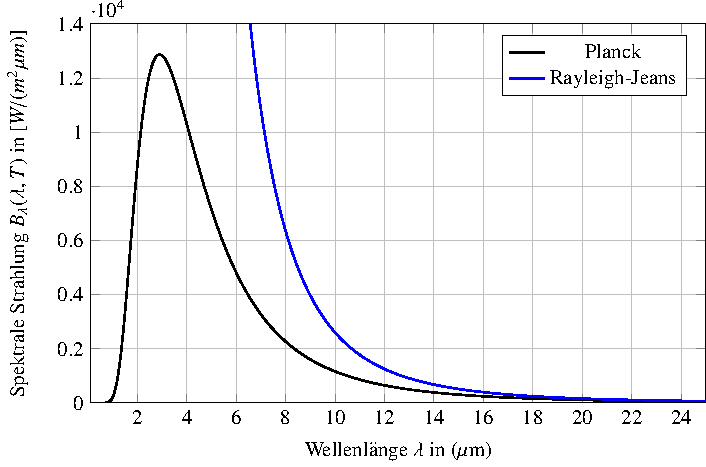
\includegraphics{papers/fourier/images/strahlung.pdf}
\caption{Vergleich der Strahlungsspektren nach Planck und nach Rayleigh–Jeans für einen auf 1000 K erhitzten Metallblock.%
\label{fourier:fig:strahlungsspektren}}
\end{figure}
	
	Planck suchte drei Jahre lang nach einer Formel, die das gemessene Spektrum des Schwarzen Körpers korrekt wiedergibt.  
	Bis dahin glaubte man, die Energie einer Welle hänge nur von ihrer Amplitude ab und Atome könnten beliebige Energiemengen abstrahlen.  
	Planck zeigte dagegen, dass die Energie einer Welle allein von ihrer Frequenz abhängt und dass Atome ihre Energie nur in diskreten Grössen abgeben können.  
	Um diese Zusammenhänge zu beschreiben, führte Planck das Wirkungsquantum $h$ ein, heute definiert als  
	$
	h = 6{,}626\cdot10^{-34}\,\mathrm{J\,s}.
	$
	Die Energie einer elektromagnetischen Welle beträgt danach $E = hf$.  
	Oft schreibt man diese Beziehung mit dem reduzierten Planckschen Wirkungsquantum $\hbar = \tfrac{h}{2\pi}$ und der Winkelfrequenz $\omega = 2\pi f$ als  
	$
	E = \hbar\,\omega = \frac{h}{2\pi}\cdot2\pi f = h f.
	$
	Auf dieser Grundlage erhielt Planck die Strahlungsdichte  
	\begin{equation}
		B(\lambda,T)
		= \frac{2\pi\,h\,c^2}{\lambda^5}\,\frac{1}{e^{\frac{h\,c}{\lambda\,k_B\,T}} - 1}
	\end{equation}
	Die Exponentialfunktion stellt sicher, dass die Intensität im Kurz­wellenbereich gegen null fällt. 
	Je höher die Frequenz, desto grösser ist das nötige Energiepaket. 
	Deshalb nimmt die Strahlung bei hohen Frequenzen wieder ab, denn hohe Frequenzen bedeuten viel Energie pro Lichtquant und es ist ziemlich unwahrscheinlich, dass ein einzelnes Atom so viel Energie auf einen Schlag abgibt. 
	Planck selbst verstand die physikalische Bedeutung dieser Quantisierung zunächst nicht, erst später wurden diese Energieportionen als Photonen erkannt.  
	Mit diesen Formel war der erste Schritt in Richtung Quantentheorie gemacht.
	Ausserdem lässt sich nun die Frage aus Kapitel~\ref{fourier:section:AnwendungAufFeld} beantworten. 
	Die Frage war, ob unendliche Frequenzen möglich sind, da bei der Fourier-Reihe die Frequenzen bis ins Unendliche ansteigen. 
	Die Antwort ist einfach mit $E = hf$ zu beantworten. Wenn die Frequenz nach Unendlich geht, so wird die Energie auch nach Unendlich gehen, was nicht möglich ist.

	
	%Einstein
	
	1905 erklärte Albert Einstein den photoelektrischen Effekt, bei dem Elektronen aus einer Metalloberfläche ausgelöst werden, sobald die einfallende elektromagnetische Strahlung eine bestimmte Mindestfrequenz überschreitet.  
	Er war der Erste, der erkannte, dass elektromagnetische Strahlung nicht nur wellenartige Eigenschaften besitzt, sondern auch in Form von Teilchen auftreten kann, die heute Photonen genannt werden.  
	Für diese Arbeit erhielt er 1921 den Nobelpreis für Physik und nicht für seine Relativitätstheorie, wie viele denken.
	
	
	%de Broglie
	
	1924 stellte Louis de Broglie eine revolutionäre Idee vor.
	Nicht nur elektromagnetische Strahlung besitzt Wellencharakter, auch Materie, also Teilchen wie Elektronen, könnten wellenartige Eigenschaften haben.
	Er vermutete, dass jedem Teilchen mit Impuls $p$ eine Wellenlänge $\lambda$ zugeordnet werden kann:
	\begin{equation}
		\lambda = \frac{h}{p}.
	\end{equation}	
	Mit dieser einfachen Formel verband de Broglie die Vorstellung von Teilchen und Wellen. Damit wurde erstmals verständlich, warum sich auch Elektronen in bestimmten Experimenten wie Wellen verhalten.
	Kurios ist, dass jedes Objekt eine Wellenlänge hat, auch ein Fussball.
	Angenommen man schiesst ein Fussball mit der Masse von 0.45 \text{kg} mit der Geschwindigkeit von 20 \text{m/s}.
	
	\begin{equation}
		\lambda = \frac{h}{p} = \frac{h}{m \cdot v} = 	\frac{6{,}626 \cdot 10^{-34} \ \text{Js}}{0{,}45 \ \text{kg} \cdot 20 \ \text{m/s}} \approx 7{,}36 \cdot 10^{-35} \ \text{m}
	\end{equation}	
	
	Die Berechnung zeigt, dass der Fussball eine extrem kleine Wellenlänge hat, somit besitzt er Wellencharakteristiken.
	Das Resultat ist absurd und hat in der Realität keinerlei Bedeutung.
	Solche Rechnungen machen nur in der Quantenwelt Sinn, auch wenn die Gleichungen für alle Objekte gelten. 
	De Broglie zeigte, dass Wellen als Teilchen intepretiert werden können und umgekehrt. 
	
	
	
	%Schrödinger
	Erwin Schrödinger formulierte 1926 eine Gleichung, die das Verhalten von Teilchen als Wellen beschreibt. 
	Sie bildet die Grundlage der Quantenmechanik. Die Lösung dieser Gleichung ist die Wellenfunktion $\psi(x, t)$. Sie liefert keine feste Bahn, sondern eine Wahrscheinlichkeitsverteilung für den Aufenthaltsort eines Teilchens.
	Die eindimensionale zeitabhängige Schrödinger-Gleichung lautet:
	
	\begin{equation}\label{fourier:equation:zeitabhaengigeSchroedingerGleichung}
		i \hbar \frac{\partial \psi(x,t)}{\partial t} = -\frac{\hbar^2}{2m} \frac{\partial^2 \psi(x,t)}{\partial x^2} + V(x) \psi(x,t)
	\end{equation}
	
	
	Um herauszufinden, wie wahrscheinlich sich ein Teilchen an einem bestimmten Ort aufhält, muss man den Betrag von $\psi(x, t)$ quadrieren. 
	Die resultierende Funktion $|\psi(x, t)|^2$ ist die Aufenthaltswahrscheinlichkeitsdichte. 
	
	Die Reise begann mit Plancks Energiepaketen, führte über Einsteins Lichtteilchen und de Broglies Materiewellen hin zu Schrödingers Wahrscheinlichkeitswellen. 
	Doch all diese Ideen behandelten Teilchen meist als isolierte Objekte.
	Die Quantenfeldtheorie geht einen Schritt weiter.
	Sie besagt, dass Teilchen nicht mehr als kleine Teilchen existieren, sondern als Anregungen von Feldern, die den gesamten Raum durchdringen. 
	Elektronen, Photonen und alle anderen Teilchen sind Wellen in ihren jeweiligen Quantenfeldern.
	Damit verschmilzt die Teilchenwelt mit der Feldvorstellung.
	Nicht das Teilchen ist grundlegend, sondern das Feld und was wir beobachten, sind nur dessen kleinste Schwingungen.
	So wird aus der Quantenmechanik eine Feldtheorie.
	
	
	Felder können durch die Kombination von einzelnen quantenmechanische harmonische Oszilatoren beschrieben werden. Solche einzelne Oszilatoren werden im nachfolgenden Kapitel angeschaut.
	
	
	\subsection{Der quantenmechanische harmonische Oszillator\label{fourier:subsection:derQMHarmonischeOszillator}}

	Im Kapitel~\ref{fourier:section:AnwendungAufFeld} wurde gezeigt, wie sich eine klassische Wellengleichung mithilfe einer Fourierzerlegung in eine Überlagerung von Schwingungsmoden zerlegen lässt.
	Jede dieser Moden erfüllt formal die Bewegungsgleichung eines klassischen harmonischen Oszillators.

	Kapitel~\ref{fourier:section:derKlassischeHarmonischeOszillator} analysierte die Gesamtenergie eines solchen Oszillators.
	Sie setzt sich zusammen aus kinetischer Energie $\frac{p^2}{2m}$ und potentieller Energie $\frac{1}{2}kx^2$, sodass sich ergibt:
	\begin{equation}\label{fourier:equation:klassischeEnergieformel}
	E = \frac{p^2}{2m} + \frac{1}{2}kx^2.
	\end{equation}

	Der nächste Schritt ist, diesen klassischen Oszillator in den quantenmechanischen Formalismus zu überführen.
	Dabei wird die klassische Energieformel (\ref{fourier:equation:klassischeEnergieformel}) zur Grundlage des sogenannten \emph{Hamilton-Operators}, der die Energie im quantenmechanischen Sinne beschreibt:
	\begin{equation}
	\hat{H} = \frac{\hat{p}^2}{2m} + \frac{1}{2} k \hat{x}^2.
	\label{fourier:equation:hamiltonOperator}
	\end{equation}
	Die klassischen Grössen Ort $x$ und Impuls $p$ werden zu \emph{Operatoren} $\hat{x}$ und $\hat{p}$.
	Diese Operatoren wirken nicht mehr auf Zahlen, sondern auf die \emph{Zustände} eines physikalischen Systems.
	
	Zur mathematischen Beschreibung dieser Zustände verwendet man den sogenannten \emph{Hilbertraum} --- ein komplexer Vektorraum, der mit einem innerem Produkt ausgestattet ist.
	Dieses innere Produkt erlaubt es, den Raum mit Begriffen wie Länge und Winkel zu versehen und somit Zustände und ihre Überlagerungen präzise zu beschreiben.
	Die Zustände selbst werden durch Vektoren in diesem Raum dargestellt.

	Die Wirkung eines Operators auf einen Zustand liefert, im Fall eines Eigenzustands, das zugehörige Messergebnis als Eigenwert.
	Die Eigenwerte des Hamilton-Operators $\hat{H}$ entsprechen den möglichen Energiezuständen des quantenmechanischen Systems.

	Ziel ist es, das \emph{Energiespektrum} des quantenmechanischen Oszillators zu bestimmen.
	Es zeigt sich, dass die Energie nur in diskreten Werten auftreten kann:
	\[
	E_n = \hbar \omega \left(n + \frac{1}{2} \right), \quad n = 0, 1, 2, \dots
	\]
	Die Herleitung dieses Spektrums erfolgt in zwei Schritten:
	\begin{itemize}
		\item Abschnitt~\ref{fourier:subsection:werkzeugeQuantenmechanik} führt die grundlegenden Werkzeuge der Quantenmechanik ein, darunter Bra-Ket-Notation, Erwartungswerte, Operatoren und die Unschärferelation.
		\item Abschnitt~\ref{fourier:subsection:Leiteroperatoren} wendet diese Konzepte auf den harmonischen Oszillator an.
		Dort werden sogenannte Leiteroperatoren eingeführt, mit deren Hilfe sich das Spektrum ableiten lässt.
	\end{itemize}
	Die Diskretisierung der Energie ist eine direkte Konsequenz der mathematischen Struktur der Theorie.
	Sie ergibt sich aus dem Operatorformalismus und wird nicht unabhängig angenommen.


	Der Grundzustand besitzt die Energie $E_0 = \frac{1}{2}\hbar \omega$.
	Die Herkunft dieses Nullpunktterms wird in Abschnitt~\ref{fourier:subsection:Leiteroperatoren} erläutert.

	Der harmonische Oszillator ist ein zentrales Modell der Quantenphysik.
	Viele physikalische Systeme lassen sich näherungsweise durch ihn beschreiben.
	Seine Quantisierung bildet die Grundlage der Quantenfeldtheorie.

	Ein wesentliches Beispiel ist das elektromagnetische Feld. Wie in Kapitel~\ref{fourier:section:AnwendungAufFeld} dargestellt, lässt es sich in Moden zerlegen, von denen jede einem quantenmechanischen Oszillator entspricht.
	Die Zustände dieser Oszillatoren --- sogenannte Photonenzahlenzustände --- erklären, warum Licht nicht kontinuierlich, sondern in diskreten Paketen (Photonen) emittiert und absorbiert wird.
	
	Auch in der Festkörperphysik und Quantenoptik ist der Oszillator zentral.
	Er beschreibt Gitterschwingungen (Phononen), Lichtfelder und Resonanzen in elektrischen Schaltungen.
	Der quantenmechanische harmonische Oszillator ist damit ein universeller Baustein in der Beschreibung quantisierter Systeme.

\subsection{Einführung in Werkzeuge der Quantenmechanik\label{fourier:subsection:werkzeugeQuantenmechanik}}
	Um die quantenmechanische Beschreibung des harmonischen Oszillators vollständig zu verstehen, ist eine neue mathematische Sprache erforderlich.
	
	In den folgenden Abschnitten werden drei zentrale Werkzeuge vorgestellt:
	\begin{itemize}
	\item \textbf{Bra-Ket-Notation}:
	Dient zur kompakten Darstellung von Zuständen und Operatoren im Hilbertraum.

	\item \textbf{Heisenbergsche Unschärferelation}:
	Beschreibt die fundamentale Grenze der gleichzeitigen Bestimmbarkeit von Ort und Impuls.

	\item \textbf{Hamilton-Operator und Schrödinger-Gleichung}:
	Zwei zentrale mathematische Werkzeuge, mit denen sich die Dynamik quantenmechanischer Systeme vollständig beschreiben lässt.
	\end{itemize}

	Diese Konzepte sind nicht nur theoretisch relevant, sondern bilden die Grundlage für das Verständnis von Photonen, Feldern und quantisierten Schwingungen im weiteren Verlauf.

	\subsubsection{Bra-Ket-Notation\label{fourier:subsubsection:braKetNotation}}
		Die Bra-Ket-Notation, auch Dirac-Notation genannt, wurde von Paul Dirac eingeführt und ist heute Standard in der Quantenmechanik.
		Sie dient dazu, Zustände und Operatoren kompakt und elegant darzustellen.
		Die Bra-Ket-Notation ist nicht nur kompakt, sondern macht viele Rechnungen in der Quantenmechanik übersichtlich und leicht handhabbar.

		\begin{itemize}
			\item Ein \emph{Ket} $|\psi\rangle$ beschreibt den Zustand eines quantenmechanischen Systems.
			Man kann sich Kets wie Richtungspfeile oder Vektoren vorstellen, die angeben, in welchem Zustand sich das System gerade befindet ---
			zum Beispiel mit welchem Energieeigenwert, welcher Spinquantenzahl oder an welchem Ort sich ein Teilchen befindet.
			\item Ein \emph{Bra} $\langle\psi|$ ist das zugehörige Dualelement zum Ket.
			Es steht symbolisch für eine Messung oder einen Test auf diesen Zustand.
			Formal ist es das komplex-konjugierte und transponierte Objekt zum Ket.
		\end{itemize}
		
		Beispiele:
		\begin{itemize}
		\item $|0\rangle$ kann den Grundzustand eines Systems beschreiben.
		\item $|x\rangle$ steht für einen Zustand, in dem sich ein Teilchen genau am Ort $x$ befindet.
		\item Allgemeine Zustände lassen sich als Superposition (Überlagerung) schreiben, beispielsweise:
		\[
			|\psi\rangle = \alpha\,|0\rangle + \beta\,|1\rangle,
		\]
		wobei $\alpha$ und $\beta$ $\in \mathbb{C}$.
		\end{itemize}

		Die Norm eines Zustands ergibt sich aus seinem Skalarprodukt mit sich selbst:
		\begin{equation}\label{fourier:equation:normEinesZustands}
			\langle \psi | \psi \rangle = \int \psi^*(x)\psi(x)dx = 1 \quad \text{(für normierte Zustände)}.
		\end{equation}
		Dabei wird der Ausdruck $\psi^*(x)\psi(x) = |\psi(x)|^2$ als \emph{Wahrscheinlichkeitsdichte} interpretiert.
		Dies bedeutet einschränkend, dass der Zustand $\psi$ immer so normiert werden muss, dass
		\begin{equation}
			\int |\psi|^2 dx = 1
		\end{equation}
		gilt.

		Das \emph{Skalarprodukt} zweier Zustände $\langle \varphi | \psi \rangle$ misst, wie ähnlich sie sich sind:
		\begin{equation}
		\langle \varphi | \psi \rangle = \int\limits_{-\infty}^{+\infty} \varphi^*(x)\,\psi(x)\,dx.
		\end{equation}
		Dazu wird die konjugiert-komplexe und transponierte Funktion $\varphi^*(x)$ mit $\psi(x)$ multipliziert und über den gesamten Raum integriert.
		Das Ergebnis ist eine einzelne (meist komplexe) Zahl, die angibt, wie stark die beiden Zustände übereinstimmen oder sich unterscheiden. 
		Dabei gilt:
		\begin{itemize}
			\item Für identische, normierte Zustände ($\varphi = \psi$) ist $\langle \psi | \psi \rangle = 1$.
			\item Sind die Zustände orthogonal, also völlig verschieden, so gilt $\langle \varphi | \psi \rangle  = 0$.
		\end{itemize}
	
	\subsubsection{Erwartungswert eines Operators\label{fourier:subsubsection:erwartungswertEinesOperators}}
		Der gemessene Durchschnittswert --- also der Erwartungswert --- eines Operators im Zustand $|\psi\rangle$ wird so berechnet:
		\begin{equation}
			\langle A \rangle = \langle \psi | A | \psi \rangle = \int \psi^*(x)\,A\,\psi(x)\,dx.
		\end{equation}
		Dieser Ausdruck ist zentral in der Quantenmechanik.
		Besonder wichtig ist er bei der Energie. Der Energieerwartungswert wird als
		\begin{equation}
			\langle H \rangle = \langle \psi|\hat{H}|\psi \rangle
		\end{equation}
		geschrieben.

		In der Dirac-Notation bezeichnet $|\psi\rangle$ den \emph{Ket}, also den Zustandsvektor des Systems.
		Der Ausdruck $\langle \psi |$ ist der zugehörige \emph{Bra}, also die komplex konjugiert transponierte Version von $|\psi\rangle$.
		Zusammen bilden sie einen sogenannten \emph{Bra-Ket} (inneres Produkt).
		Dabei gilt:
		\begin{itemize}
			\item Der Operator $A$ wirkt zunächst auf den Ket $|\psi\rangle$, also auf die Wellenfunktion $\psi(x)$ von rechts.
			\item Anschliessend wird das Ergebnis mit dem Bra $\langle \psi|$ bzw. der komplex-konjugierten Wellenfunktion $\psi^*(x)$ multipliziert.
			\item Durch Integration über alle Orte $x$ erhält man den Mittelwert --- den Erwartungswert.
		\end{itemize}
		Das Ergebnis $\langle A \rangle$ ist also der theoretische Durchschnittswert, den man bei vielen Messungen der Grösse $A$ im Zustand $|\psi\rangle$ erhält.

		Wenn der Zustand $|\psi\rangle$ ein \emph{Eigenzustand} des Operators $\hat{A}$ ist, dann gilt:
		\begin{equation}
			\hat{A} | \psi \rangle = a | \psi \rangle \Rightarrow \langle A \rangle = a.
		\end{equation}
		Dabei ist $a$ der \emph{Eigenwert}, der dem Eigenzustand $|\psi\rangle$ des Operators $\hat{A}$ zugeordnet ist. 
		Man erhält also bei jeder Messung denselben Wert a, was typisch für beispielsweise einen stationären Energiezustand ist.

	\subsubsection{Heisenbergs Unschärferelation%
	\label{fourier:subsubsection:unschaerferelation}}
		In der klassischen Mechanik lassen sich Ort $x$ und Impuls $p$ gleichzeitig beliebig genau messen.
		In der Quantenmechanik ist dies \emph{grundsätzlich nicht möglich}.
		Der Impulsoperator lautet:
		\begin{equation}
			\hat{p} = \frac{\hbar}{i} \frac{d}{dx}.
		\end{equation}
		Man kann nicht einfach sagen ``Das Teilchen hat genau diesen Impuls'', sondern der Impuls ist grundsätzlich unscharf (nicht exakt bestimmbar).
		Ort und Impuls sind sogenannte nicht gleichzeitig messbare Grössen:
		Ihre Operatoren ``vertauschen'' nicht miteinander, was mathematisch ausgedrückt wird durch
		\begin{equation}
			[\hat{x},\hat{p}] = \hat{x} \hat{p} - \hat{p} \hat{x} = i \hbar.
		\end{equation}
		Diese fehlende Vertauschbarkeit führt direkt zur bekannten Unschärferelation.
		Ihre Herleitung basiert auf einer grundlegenden mathematischen Ungleichung, der sogenannten \emph{Cauchy-Schwarz-Ungleichung}:
		\begin{equation}\label{fourier:equation:CauchySchwarzUngleichung}
			\vec{a} \bullet \vec{b} = |\vec{a}| |\vec{b}|\cos\alpha \le |\vec{a}| |\vec{b}|.
		\end{equation}
		die besagt, dass das Skalarprodukt zweier Vektoren nie grösser sein kann als das Produkt ihrer Längen.
		Übertragen auf die Wellenfunktionen zweier Quantenzustände $|\varphi\rangle$ und $|\chi\rangle$, erhält man
		\begin{equation}
			|\langle\varphi | \chi\rangle|^2 \le \langle\varphi | \varphi\rangle \langle\chi | \chi\rangle.
		\end{equation}
		Diese Relation setzt eine obere Schranke dafür, wie stark zwei Zustände miteinander überlappen können. Sie beschreibt also, wie ähnlich sich zwei Zustände in ihrer quantenmechanischen Beschreibung überhaupt sein können.
		Der Ausdruck $|\langle\varphi|\chi\rangle|^2$ misst die Überlappung der beiden Zustände, also gewissermassen, wie ähnlich sie sich sind.
		Die Terme $\langle\varphi|\varphi\rangle$ und $\langle\chi|\chi\rangle$ entsprechen dabei den Quadraten der Längen (Normen) der Zustände.
		Der Betrag des Skalarprodukts kann also niemals grösser werden als das Produkt der Normen, ganz analog zur klassischen Vektoranalysis.
		Das Quadrat auf der linken Seite ergibt sich, weil die Ungleichung eine Aussage über den Betrag des Skalarprodukts ist, während die rechte Seite stets reell und positiv ist.
		Diese Form der Ungleichung bildet die mathematische Grundlage für die Herleitung der heisenbergschen Unschärferelation.
		Die Zustände $|\varphi\rangle$ und $|\chi\rangle$ sind hier in der Bra-Ket-Notation geschrieben, einer kompakten Notation für Zustände in der Quantenmechanik, wie sie in Abschnitt~\ref{fourier:subsubsection:braKetNotation} eingeführt wurde.

		Setzt man
		\begin{equation}
			|\varphi\rangle = (\hat{x} - \langle \hat{x} \rangle) |\psi\rangle \quad |\chi\rangle = (\hat{p} - \langle \hat{p} \rangle) | \psi\rangle,
		\end{equation}
		also die Abweichungen von Ort und Impuls gegenüber ihren Mittelwerten ein, so führen die Definitionen
		\begin{equation}
			\sigma_x^2 = \langle\varphi | \varphi\rangle \text{ und } \sigma_p^2 = \langle\chi | \chi\rangle
		\end{equation}
		für die sogenannten Standardabweichungen --- ein Mass für die „Streuung“ oder Unschärfe --- zusammen mit der Vertauschungsrelation
		\begin{equation}
			\langle\psi | [\hat{x},\hat{p}] | \psi\rangle = i\hbar
		\end{equation}
		und der Cauchy-Schwarz-Ungleichung (\ref{fourier:equation:CauchySchwarzUngleichung}) zur Beziehung:
		\begin{equation}
			\sigma_x^2 \sigma_p^2 \ge \frac{1}{4} |\langle\psi | [\hat{x},\hat{p}] | \psi\rangle|^2 = \frac{\hbar^2}{4}.
		\end{equation}
		Nimmt man aus beiden Seiten die Quadratwurzel, erhält man die bekannte Form der Unschärferelation:
		\begin{equation}\label{fourier:equation:FormUnschaerferelation}
			\sigma_x \sigma_p \ge \frac{\hbar}{2}.
		\end{equation}

		Hier bedeuten $\sigma_x$ und $\sigma_p$ die Unschärfen (Standardabweichungen) in Ort und Impuls.
		Die Unschärferelation sagt also:
		Je genauer der Ort eines Teilchens bekannt ist (kleines $\sigma_x$), desto unschärfer muss sein Impuls ($\sigma_p$) sein --- und umgekehrt.
		Das zeigt anschaulich die Wellennatur von Teilchen:
		Ein Teilchen, das genau lokalisiert ist, muss eine breite Wellenverteilung im Impulsraum haben.
		Würde man das $\tfrac{1}{2}$ in der Form der Unschärferelation (\ref{fourier:equation:FormUnschaerferelation}) weglassen, erhielte man eine vereinfachte, aber weniger präzise Darstellung des Zusammenhangs.

		Die Unschärferelation macht deutlich, dass klassische Begriffe wie ``Ort'' und ``Impuls'' in der Quantenmechanik nur noch als mittlere Werte und Streuungen auftreten können.
		Um diese Konzepte mathematisch präzise zu fassen und weiterführende Aussagen über die Dynamik eines Systems zu treffen, bedarf es weiterer Werkzeuge ---
		insbesondere des Hamilton-Operators und der Schrödinger-Gleichung.

	\subsubsection{Hamilton-Operator und Schrödinger-Gleichung%
	\label{fourier:subsubsection:hamiltonOperatorUndSchroedinger}}
		Die Unschärferelation hat gezeigt, dass Ort und Impuls eines Teilchens nicht gleichzeitig beliebig genau bestimmt werden können.
		Diese fundamentale Eigenschaft ist nicht nur eine Aussage über Messprozesse,
		sondern hat unmittelbare Konsequenzen für die Dynamik eines quantenmechanischen Systems.
		Um zu beschreiben, wie sich ein solcher Zustand mit der Zeit entwickelt,
		benötigt man ein mathematisches Werkzeug, das diese Unschärfe respektiert
		und gleichzeitig Auskunft über die Energieverhältnisse im System gibt.
		
		Dieses Werkzeug ist der Hamilton-Operator \( \hat{H} \).
		Er spielt in der Quantenmechanik eine doppelte Rolle:
		\begin{itemize}
		\item Er beschreibt die Gesamtenergie eines Systems (kinetisch und potentiell).
		\item Er steuert die zeitliche Entwicklung eines Zustands über die Schrödinger-Gleichung.
		\end{itemize}
		Im Abschnitt~\ref{fourier:subsection:derQMHarmonischeOszillator} wurde $\hat{H}$ bereits in einem konkreten Beispiel eingeführt.
		Hier betrachten wir ihn unabhängig von einem speziellen Potential.
		In der klassischen Mechanik ergibt sich die Gesamtenergie aus der Summe von kinetischer und potentieller Energie.
		In der Quantenmechanik wird diese Grösse durch den Hamilton-Operator:
		\begin{equation}\label{fourier:equation:HamiltonOperatorQM}
			\hat{H} = \frac{\hat{p}^2}{2m} + V(\hat{x})
		\end{equation}
		ersetzt.
		Dabei treten $\hat{x}$ und $\hat{p}$ als nicht-kommutierende (also nicht vertauschbare) Operatoren auf.
		
		In der Ortsdarstellung gilt:
		\begin{equation}
			\hat{x} = x, \qquad \hat{p} = -i\hbar \frac{\partial}{\partial x}
		\end{equation}
		Setzt man dies ein, ergibt sich die konkrete Form des Hamilton-Operators:
		\begin{equation}
			\hat{H} = -\frac{\hbar^2}{2m} \frac{\partial^2}{\partial x^2} + V(x)
		\end{equation}
		Dieser Operator ist zentral in der zeitabhängigen Schrödinger-Gleichung (\ref{fourier:equation:zeitabhaengigeSchroedingerGleichung}):
		\begin{equation}
			i\hbar \frac{\partial}{\partial t} \psi(x,t) = \hat{H} \psi(x,t)
		\end{equation}
		Sie beschreibt, wie sich der Zustand eines Systems mit der Zeit verändert.
		Die Lösung dieser Gleichung ist die sogenannte Wellenfunktion \( \psi(x,t) \).

		Gleichzeitig ist der Hamilton-Operator ein sogenannter Observablen-Operator.
		Das bedeutet:
		Seine Eigenwerte entsprechen den möglichen Energie-Messwerten des Systems.
		Und seine Eigenfunktionen beschreiben stationäre Zustände mit konstanter Energie.
		Ein weiterer wichtiger Punkt ist, dass die Struktur von \( \hat{H} \) direkt von den Vertauschungsrelationen von \( \hat{x} \) und \( \hat{p} \) abhängt:
		\begin{equation}
			[\hat{x}, \hat{p}] = i \hbar
		\end{equation}

		Diese Beziehung führt, wie gesehen, zur Unschärferelation.
		Gleichzeitig stellt sie sicher, dass die Dynamik mit den Regeln der Quantenmechanik verträglich ist.
		Die mathematische Konsistenz der Schrödinger-Gleichung hängt also von genau dieser Nichtvertauschbarkeit ab.

		Beispielhaft kann man mit dem Hamilton-Operator Erwartungswerte berechnen.
		Für den Impuls ergibt sich:
		\begin{equation}
			E(p) = \int \bar{\psi}(x) \, \hat{p} \, \psi(x) \, dx 
			= \int \bar{\psi}(x) \, \frac{\hbar}{i} \, \frac{\partial \psi}{\partial x} \, dx 
			= \langle \psi | \hat{p} | \psi \rangle
		\end{equation}


		Solche Berechnungen sind nicht nur theoretisch relevant, sondern liefern konkrete Vorhersagen für Experimente.
		Sie zeigen, wie Operatoren mit Zuständen kombiniert werden, um physikalische Grössen wie Energie, Ort oder Impuls zu berechnen.

		Der Hamilton-Operator steht somit im Zentrum der quantenmechanischen Theorie.
		Er fasst die Energie- und Dynamikstruktur eines Systems in einem einzigen Objekt zusammen.

	\subsubsection{Ausblick\label{fourier:subsubsection:Ausblick}}
		Mit den bisher eingeführten Werkzeugen lässt sich der quantenmechanische harmonische Oszillator vollständig verstehen.
		Im nächsten Abschnitt wird gezeigt, wie sich der Hamilton-Operator in diesem Fall besonders elegant mithilfe sogenannter \emph{Leiteroperatoren} behandeln lässt.

		Dabei wird betrachtet, wie diese Operatoren auf Zustände wirken, wie daraus die \emph{Energieniveaus} entstehen ---
		und warum der Oszillator niemals die Energie Null haben kann.

	\subsection{Leiteroperatoren\label{fourier:subsection:Leiteroperatoren}}
		Die Energie des quantenmechanischen harmonischen Oszillators ist diskret.
		Ziel dieses Abschnitts ist es, diese Aussage formal zu begründen.
		Grundlage ist die algebraische Methode mit sogenannten Leiteroperatoren, die eine vollständige Lösung des Systems ermöglichen, ohne Differentialgleichungen zu lösen.	

		\subsubsection{Dimensionlose Operatoren\label{fourier:subsubsection:DimensionsloseOperatoren}}
			Zur Vereinfachung führt man dimensionslose Operatoren ein:
			\[
				Q = \sqrt{\frac{m\omega}{\hbar}}x
				\qquad\text{und}\qquad
				P = \frac{1}{\sqrt{m\hbar\omega}}p.
			\]
			Die Wurzelausdrücke sorgen dafür, dass beide Operatoren keine physikalischen Einheiten mehr haben.
			Der Hamilton-Operator~\ref{fourier:equation:HamiltonOperatorQM} des harmonischen Oszillators nimmt damit die Form an:
			\begin{equation}\label{fourier:equation:HamiltonOperatorDimLos}
				H = \frac{1}{2}(P^2 + Q^2).
			\end{equation}

		\subsubsection{Definition der Leiteroperatoren\label{fourier:subsubsection:DefinitionLeiteroperatoren}}
			Der Ausdruck~\ref{fourier:equation:HamiltonOperatorDimLos} lässt sich faktorisieren:
			\[
				H = \frac{1}{2}(Q + iP)(Q - iP).
			\]
			Dies motiviert die Definition der Leiteroperatoren:
			\begin{equation}
				a = \frac{1}{\sqrt{2}}(Q + iP),
				\qquad\text{und}\qquad
				a^+ = \frac{1}{\sqrt{2}}(Q - iP).
			\end{equation}
			Diese erfüllen die fundamentale Vertauschungsrelation:
			\begin{equation}
				[a, a^+] = 1.
			\end{equation}
			Die Reihenfolge der Operatoren ist entscheidend: $[a^+, a] = -1$.
			\textit{Anmerkung:}
			Ursprünglich wurde der Erzeugungsoperator mit einem $\dagger$ (engl. „dagger“) als hochgestelltes Symbol geschrieben, also $a^\dagger$.
			Aufgrund der begrenzten Verfügbarkeit von Sonderzeichen auf Tastaturen und in einfachen Textsystemen wird oft stattdessen das Pluszeichen $a^+$ verwendet.
			Heute findet man deshalb in der Literatur häufig das hochgestellte Plus.
			Beide Bezeichnungen meinen denselben Operator.

		\subsubsection{Hamilton-Operator in Operatorform\label{fourier:subsubsection:HamiltonOperatorInOperatorform}}
			Die Leiteroperatoren ermöglichen eine kompakte Darstellung des Hamilton-Operators.
			Zunächst ergibt sich durch Ausmultiplizieren:
			\[
				a^+a = \frac{1}{2}(Q - iP)(Q + iP) = \frac{1}{2}(Q^2 + iQP - iPQ + P^2) = \frac{1}{2}(Q^2 + P^2 + i[Q, P]).
			\]
			Da $QP - PQ = [Q, P] = i$, folgt:
			\[
				a^+a = \frac{1}{2}(Q^2 + P^2 - 1).
			\]
			Formt man diese Gleichung nach $Q^2 + P^2$ um, erhält man:
			\[
				Q^2 + P^2 = 2a^+a + 1.
			\]
			Setzt man dies in den ursprünglichen Hamilton-Operator ein, ergibt sich
			\[
				H = \frac{1}{2}(Q^2 + P^2) = \frac{1}{2}(2a^+a + 1) = a^+a + \frac{1}{2}.
			\]
			Mit Einheiten eingesetzt:
			\begin{equation}
				\hat{H} = \hbar\omega \left(a^+ a + \frac{1}{2}\right) = \hbar\omega \left(N + \frac{1}{2}\right).
			\end{equation}
			Hierbei ist $N = a^+a$ der sogenannte Zahloperator.
			Er zählt die Anzahl von Quanten (zum Beispiel Photonen) im Zustand.
			Der Term $\frac{1}{2}\hbar\omega$ ergibt sich aus der Vertauschungsrelation und beschreibt die \emph{Nullpunktsenergie} des Oszillators.
		
		\subsubsection{Wirkung der Leiteroperatoren\label{fourier:subsubsection:WirkungLeiteroperatoren}}
			Die gemessene Energie eines quantenmechanischen Zustands ist der Erwartungswert des Hamilton-Operators:
			\begin{equation}
				\langle\psi|\hat{H}|\psi\rangle = \langle\psi|E|\psi\rangle.
			\end{equation}
			Gilt $|\psi\rangle$ als Eigenzustand von $\hat{H}$ mit Eigenwert $E$, so folgt:
			\[
				\hat{H}|\psi\rangle = E|\psi\rangle.
			\]
			Weil $E$ nur eine Zahl ist, lässt sich der Ausdruck vereinfachen:
			\[
				\langle\psi|E|\psi\rangle = E \langle\psi|\psi\rangle.
			\]
			Für normierte Zustände gilt $\langle\psi|\psi\rangle = 1$ (siehe Formel~\ref{fourier:equation:normEinesZustands}), womit sich
			\[
				E \langle\psi|\psi\rangle = E \cdot 1 = E
			\]
			ergibt.
			Der Erwartungswert der Energie ist also gleich dem Eigenwert, wenn der Zustand $|\varphi\rangle$ ein Eigenzustand des Hamilton-Operators ist.
			
			Das heisst, man kann jetzt ausrechnen, wie $a$ und $a^+$ die Energie ändern.
			Zunächst verwenden wir die Vertauschungsrelationen:
			\[
				[H, a^+] = \hbar\omega a^+
				\qquad
				und
				\qquad
				[H, a] = -\hbar\omega a
			\]
			Daraus folgt:
			\[
				H a^+ |\psi_n\rangle = a^+ H|\psi_n\rangle + [H, a^+]|\psi_n\rangle = a^+ E_n|\psi_n\rangle + \hbar\omega a^+ |\psi_n\rangle = (E_n + \hbar\omega)a^+|\psi_n\rangle
			\]
			und
			\[
				H a|\psi_n\rangle = a H|\psi_n\rangle + [H, a]|\psi_n\rangle = a E_n|\psi_n\rangle - \hbar\omega a|\psi_n\rangle = (E_n - \hbar\omega)a|\psi_n\rangle
			\]
			Also:
			\begin{equation}
				H a^+ |\psi_n\rangle =  (E_n + \hbar\omega)a^+ |\psi_n\rangle \quad \text{(mehr Energie)}
			\end{equation}
			\begin{equation}
				H a |\psi_n\rangle = (E_n - \hbar\omega)a | \psi_n\rangle \quad \text{(weniger Energie)}
			\end{equation}
			Das zeigt, dass der Erzeugungsoperator $a^+$ die Energie um $\hbar\omega$ erhöht, während der Vernichtungsoperator $a$ sie um $\hbar\omega$ verringert.

			Die Operatoren $a^+$ (Erzeugungsoperator) und $a$ (Vernichtungsoperator) verändern die Teilchenzahl der Zustände:
			\[
				a^+|\psi_n\rangle = \sqrt{n+1}\,|\psi_\text{n+1}\rangle,
				\qquad
				a|\psi_n\rangle = \sqrt{n}\,|\psi_\text{n-1}\rangle.
			\]
			Dabei wird der Erzeugungsoperator $a^+$ auf die Wellenfunktion $|\psi_n\rangle$ angewendet und hebt den Zustand auf das nächsthöhere Energieniveau $|\psi_{n+1}\rangle$ an.
			Umgekehrt senkt der Vernichtungsoperator $a$ den Zustand um ein Energieniveau auf $|\psi_{n-1}\rangle$.
			
			\textit{Bemerkung:} 
			Die Wurzeln entstehen aus der Normierung der Zustände.
			Die Faktoren $\sqrt{n+1}$ beziehungsweise $\sqrt{n}$ sorgen dafür, dass die Zustände $|\psi_{n\pm1}\rangle$ korrekt normiert bleiben, wenn die Operatoren wirken.
			Ohne diese Faktoren würde sich die Länge (Norm) der Zustände verändern.
			Dies bedeutet:
			\begin{itemize}
				\item Der Operator $a^+$ erhöht die Quantenzahl $n$ um eins – er \textbf{erzeugt} also ein zusätzliches Quant (z.\,B. ein Photon).
				\item Der Operator $a$ senkt die Quantenzahl $n$ um eins – er \textbf{vernichtet} ein Quant.
			\end{itemize}

			Diese Operatoren erlauben eine elegante algebraische Beschreibung der Quantenzustände, ohne dass komplexe Differentialgleichungen gelöst werden müssen.

		\subsubsection{Energieeigenwerte\label{fourier:subsubsection:Energieeigenwerte}}
			Da $\hat{H} = \hbar\omega(N + \frac{1}{2})$, folgt:
			\begin{equation}
				H\,|\psi_n\rangle = \hbar\omega\left(n + \frac{1}{2}\right) |\psi_n\rangle.
			\end{equation}
			Die Eigenwerte sind also diskret:
			\[
				E_n = \hbar\omega\left(n + \frac{1}{2}\right), \quad \text{mit } n = 0,1,2,\dots
			\]
			Der Zustand mit $n = 0$ ist der Grundzustand mit minimaler Energie $\frac{1}{2}\hbar\omega$.
			Zustände mit negativer Teilchenzahl existieren nicht, da sonst unphysikalisch negative Energien entstünden.

		\subsubsection{Bedeutung für die Quantisierung des Lichts\label{fourier:subsubsection:QuantisierungElmagFeld}}
			Diese Struktur überträgt sich direkt auf die Quantisierung des elektromagnetischen Feldes.
			Jede Modenkombination eines Feldes (Frequenz, Richtung, Polarisation) wird als unabhängiger Oszillator modelliert.
			Die zugehörigen Fourier-Koeffizienten verhalten sich wie die Operatoren $a$ und $a^+$.

			Die Energie des Feldes ergibt sich analog:
			\[
				E_n = \hbar\omega\left(n + \frac{1}{2}\right),
			\]
			was zur quantisierten Natur des Lichts  führt.
			Das Photon entspricht einem einzelnen Quant der Energie $\hbar\omega$.
			Jeder Zustand $n$ enthält $n$ Photonen.
			
			\textit{Anmerkung zur Polarisation:}
			Jede Polarisation entspricht einem eigenen Oszillator mit eigenen Leiteroperatoren.
			Reales Licht besteht aus Überlagerungen dieser Moden.

		\subsubsection{Bemerkung zu Energiegrenzen\label{fourier:subsubsection:BemerkungBegrenztheitDerEnergie}}
			Der Vernichtungsoperator $a$ kann nur bis zum Grundzustand angewendet werden.
			Eine weitere Anwendung würde unphysikalische Zustände erzeugen.
			Nach oben existiert formal kein Limit, allerdings setzt die reale Physik praktische Grenzen (beispielsweise durch Wechselwirkungen, Instabilität oder Gravitationseffekte bei extremer Energiedichte).

		\subsubsection{Messung von Energie\label{fourier:subsubsection:MessungQuantisierterEnergie}}
			Die Energie eines Systems wird über den Erwartungswert des Hamilton-Operators gemessen:
			\begin{equation}
				\langle\varphi|\hat{H}|\varphi\rangle = E.
			\end{equation}
			Für Eigenzustände gilt:
			\begin{equation}
				\hat{H}|\varphi_n\rangle = E_n|varphi_n\rangle.
			\end{equation}
			Durch Anwendung von $a$ oder $a^+$ auf $|\varphi_n\rangle$ wird der Zustand in ein höheres oder tieferes Energieniveau verschoben:
			\[
				\hat{H}a^+|\varphi_n\rangle = E_\text{n+1}a^+|\varphi_n\rangle, \qquad \hat{H}a|\varphi_n\rangle = E_\text{n-1}a|\varphi_n\rangle.
			\]
			Diese algebraische Struktur beschreibt den Übergang zwischen diskreten Energieniveaus, wie der etwa bei der Emission oder Absorption einzelner Quanten (beispielsweise Photonen) auftritt.

\section{Fazit\label{fourier:section:fazit}}
\kopfrechts{Fazit}
	In diesem Kapitel wurde der Zusammenhang zwischen der klassischen Fourier-Analyse und der Quantenmechanik dargestellt.
	Es wurde gezeigt, wie komplexe Schwingungen durch Fourier-Reihen in einfachere harmonische Komponenten zerlegt werden können.

	Am Beispiel des quantenmechanischen harmonischen Oszillators wurden die Leiteroperatoren $a^+$ und $a$ eingeführt.
	Diese Operatoren entsprechen der Addition beziehungsweise Subtraktion eines diskreten Energiequants $\hbar \omega$.
	Damit wird das grundlegende Prinzip der Quantisierung veranschaulicht, dass Energie nicht kontinuierlich, sondern in diskreten Stufen vorkommt.

	Die Zustände $|\psi_n\rangle$ des Oszillators stellen diskrete Energieeigenzustände dar, deren Energiewerte durch ganzzahlige Vielfache von $\hbar \omega$ bestimmt sind.
	Dieses Konzept ist grundlegend für viele quantenmechanische Systeme und findet Anwendung in verschiedenen Bereichen der Physik, die Schwingungs- und Wellenphänomene beschreiben.

	Für weiterführende mathematische Details und eine vertiefte Behandlung der Quantisierung kann Kapitel 8 in~\cite{fourier:quantenmechanik} konsultiert werden.

	Zusammenfassend lässt sich festhalten, dass Schwingungen und Energie in der Quantenmechanik in diskreten Quantensprüngen auftreten, was einen wesentlichen Unterschied zur klassischen Physik darstellt.
